\section{Results}

We evaluate Q-learning and Floyd-Warshall Reinforcement Learning (FWRL)  on two
metrics in two different environments. The two metrics we use are Latency Ratio
and average reward per episode. The Latency ratio metric was introduced in
\citet{MiPaViICLR2017}, which is defined as the ratio of time taken to reach the
goal for the first to time to the average time taken to hit the goal thereafter.
The Latency ratio thus measures the ratio of exploration time for first time
finding the goal to the average exploitation time to reach the goal. Hence,
higher latency ratio is better.
Fig~\ref{fig:ql-fw-grid-world-results} and
Fig~\ref{fig:ql-fw-windy-world-results} show the results.

\begin{figure}%
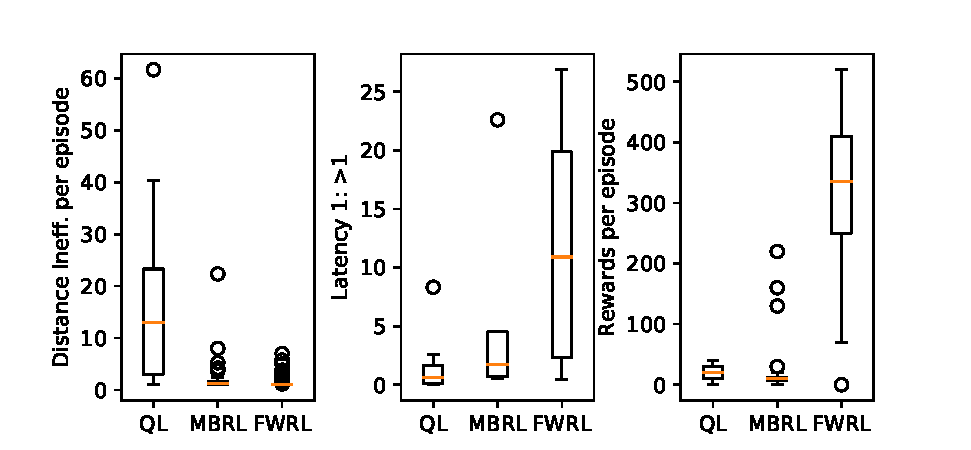
\includegraphics[width=\columnwidth]{./media/metrics-grid-world.pdf}\\
\caption{Results on grid world. FWRL beats Q-Learning consistently. Higher is
  better in both the metrics (higher is better).}
\label{fig:ql-fw-grid-world-results}%
\end{figure}
\begin{figure}
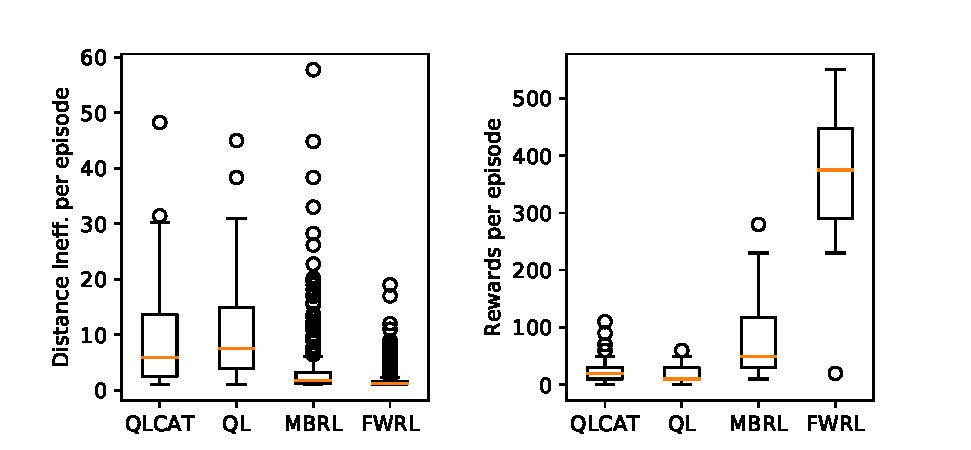
\includegraphics[width=\columnwidth]{./media/metrics-windy-world.pdf}%
\caption{Results on windy world. FWRL beats Q-Learning consistently. Higher is
  better in both the metrics (higher is better).}
\label{fig:ql-fw-windy-world-results}%
\end{figure}
